%%%%%%%%%%%%%%%%%%%%%%%%%%%%%%%%%%%%%%%%%
% Beamer Presentation
% LaTeX Template
% Version 1.0 (10/11/12)
%
% This template has been downloaded from:
% http://www.LaTeXTemplates.com
%
% License:
% CC BY-NC-SA 3.0 (http://creativecommons.org/licenses/by-nc-sa/3.0/)
%
%%%%%%%%%%%%%%%%%%%%%%%%%%%%%%%%%%%%%%%%%

%----------------------------------------------------------------------------------------
%	PACKAGES AND THEMES
%----------------------------------------------------------------------------------------

\documentclass[aspectratio=169]{beamer}

\mode<presentation> {

% The Beamer class comes with a number of default slide themes
% which change the colors and layouts of slides. Below this is a list
% of all the themes, uncomment each in turn to see what they look like.

%\usetheme{default}
%\usetheme{AnnArbor}
%\usetheme{Antibes}
%\usetheme{Bergen}
%\usetheme{Berkeley}
%\usetheme{Berlin}
%\usetheme{Boadilla}
%\usetheme{CambridgeUS}
%\usetheme{Copenhagen}
%\usetheme{Darmstadt}
%\usetheme{Dresden}
%\usetheme{Frankfurt}
%\usetheme{Goettingen}
%\usetheme{Hannover}
%\usetheme{Ilmenau}
%\usetheme{JuanLesPins}
%\usetheme{Luebeck}
\usetheme{Madrid}
%\usetheme{Malmoe}
%\usetheme{Marburg}
%\usetheme{Montpellier}
%\usetheme{PaloAlto}
%\usetheme{Pittsburgh}
%\usetheme{Rochester}
%\usetheme{Singapore}
%\usetheme{Szeged}
%\usetheme{Warsaw}

% As well as themes, the Beamer class has a number of color themes
% for any slide theme. Uncomment each of these in turn to see how it
% changes the colors of your current slide theme.

%\usecolortheme{albatross}
%\usecolortheme{beaver}
%\usecolortheme{beetle}
%\usecolortheme{crane}
%\usecolortheme{dolphin}
%\usecolortheme{dove}
%\usecolortheme{fly}
%\usecolortheme{lily}
%\usecolortheme{orchid}
%\usecolortheme{rose}
%\usecolortheme{seagull}
%\usecolortheme{seahorse}
%\usecolortheme{whale}
%\usecolortheme{wolverine}

%\setbeamertemplate{footline} % To remove the footer line in all slides uncomment this line
%\setbeamertemplate{footline}[page number] % To replace the footer line in all slides with a simple slide count uncomment this line

%\setbeamertemplate{navigation symbols}{} % To remove the navigation symbols from the bottom of all slides uncomment this line
}

\usepackage{graphicx} % Allows including images
\usepackage{booktabs} % Allows the use of \toprule, \midrule and \bottomrule in tables

\usepackage{siunitx}
\usepackage{caption}
\usepackage{subcaption}

%----------------------------------------------------------------------------------------
%	TITLE PAGE
%----------------------------------------------------------------------------------------

\title[CRT]{Preliminary research on an electron beam setup for the QUAK experiment} % The short title appears at the bottom of every slide, the full title is only on the title page

\author{Frank Ebel\\ Alexander Preimesberger} % Your name
\institute[TU] % Your institution as it will appear on the bottom of every slide, may be shorthand to save space
{
TU Wien \\ % Your institution for the title page
\medskip
01429282\\ 01427641
}
\date{15. March 2021} % Date, can be changed to a custom date

\begin{document}

\begin{frame}
\titlepage % Print the title page as the first slide
\end{frame}

\begin{frame}
\frametitle{Overview} % Table of contents slide, comment this block out to remove it
\tableofcontents % Throughout your presentation, if you choose to use \section{} and \subsection{} commands, these will automatically be printed on this slide as an overview of your presentation
\end{frame}

%----------------------------------------------------------------------------------------
%	PRESENTATION SLIDES
%----------------------------------------------------------------------------------------

%------------------------------------------------
\section{CRT} % Sections can be created in order to organize your presentation into discrete blocks, all sections and subsections are automatically printed in the table of contents as an overview of the talk
%------------------------------------------------

\subsection{Characterization} % A subsection can be created just before a set of slides with a common theme to further break down your presentation into chunks

\begin{frame}
	\frametitle{Characterization}
	\begin{itemize}
		\item Model Heerlen D14-363GY/123
		\item Voltage \SI{2}{\kilo\volt}
		\item Filament heating voltage \SI{\approx 6}{\volt}
		\item Metal oxide cathode with barium-, strontium-, and possibly aluminum-oxide
	\end{itemize}
\end{frame}

%------------------------------------------------

\begin{frame}
	\frametitle{CRT}
	\begin{figure}
		\centering
		\begin{subfigure}{.4\textwidth}
			\centering
			\includegraphics[width=.65\textwidth]{../Chapters/CRT-Basics/CRT.JPG}
		\end{subfigure}%
		\begin{subfigure}{.4\textwidth}
			\centering
			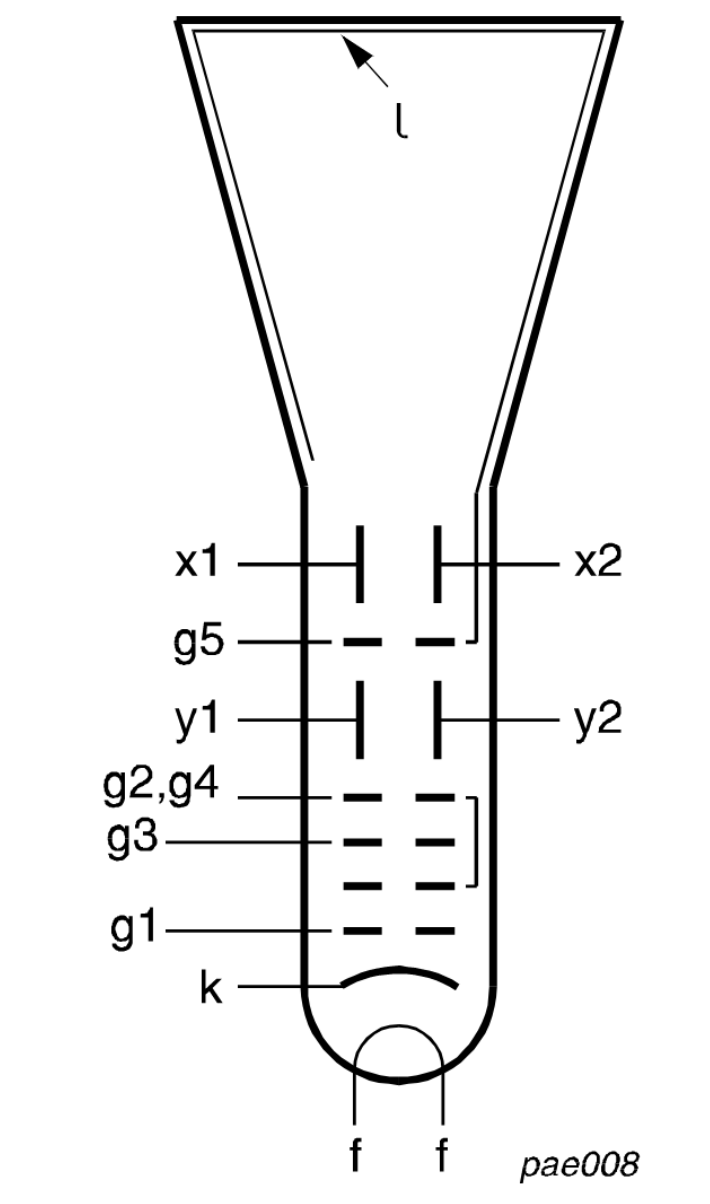
\includegraphics[width=.65\textwidth]{../Chapters/CRT-Basics/electrode configuration.png}
		\end{subfigure}
	\end{figure}
\end{frame}

%------------------------------------------------

\begin{frame}
	\frametitle{Cathode SEM image}
	\begin{figure}
		\centering
		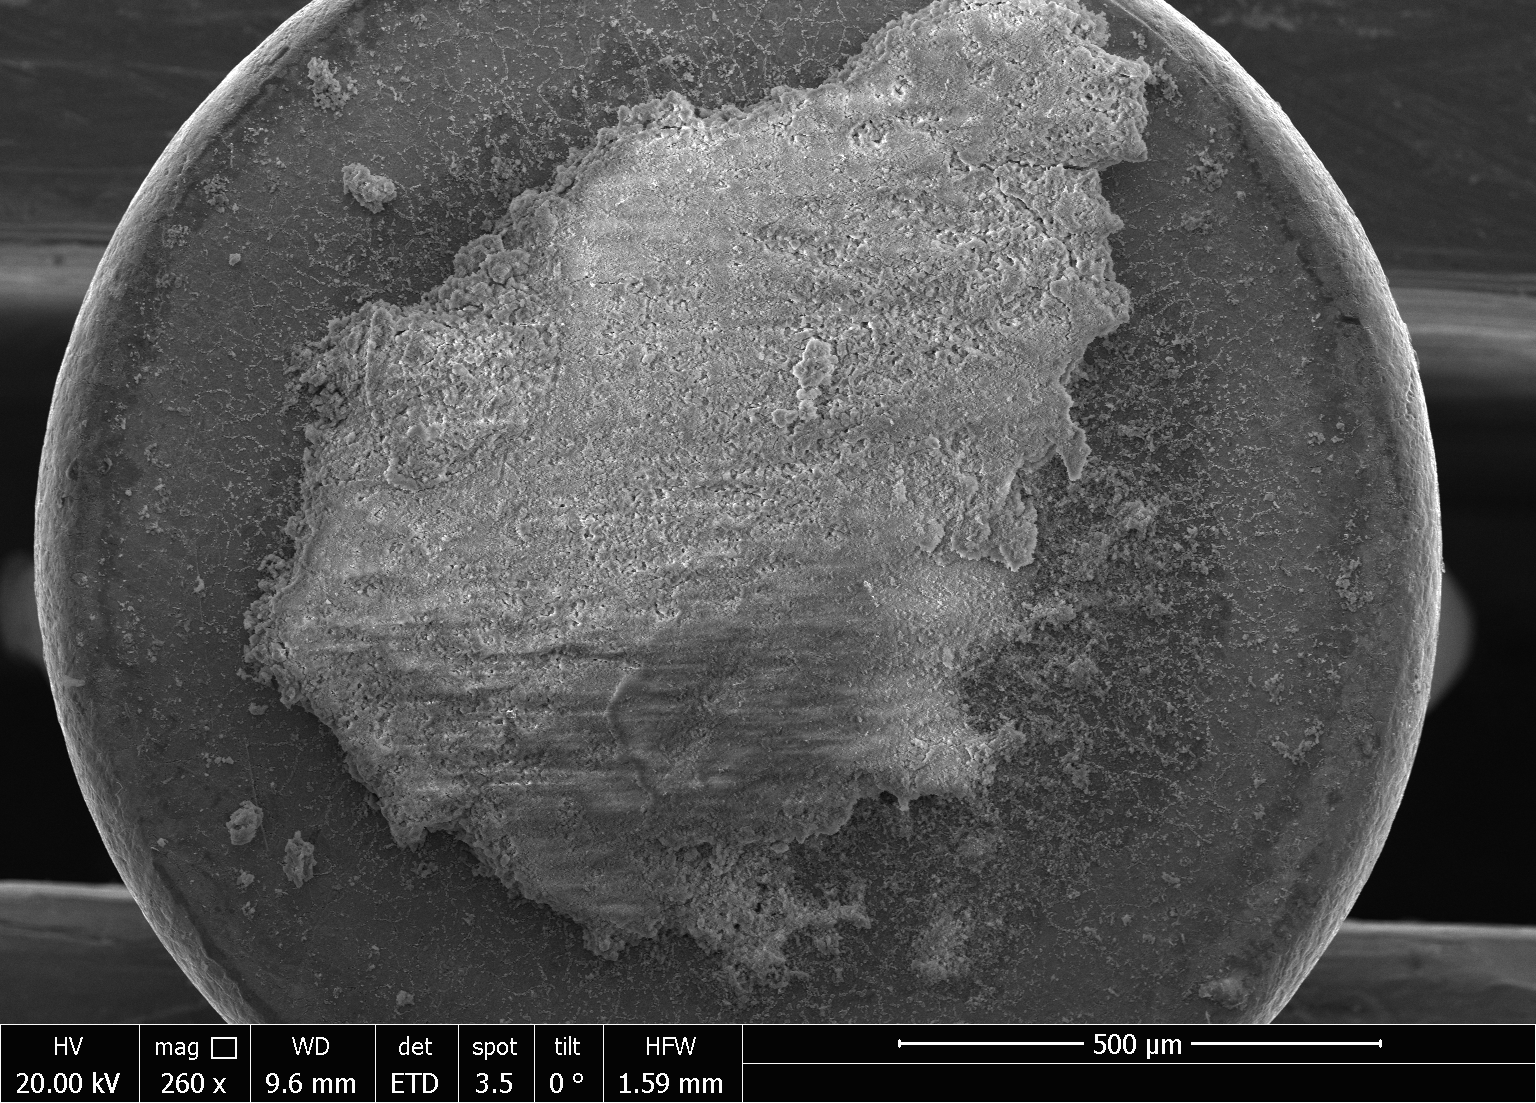
\includegraphics[width=0.65\textwidth]{../Chapters/CRT-Basics/SEM_image.png}
	\end{figure}
\end{frame}

%------------------------------------------------

\begin{frame}
	\frametitle{Heater}
	\begin{figure}[ht]
		\centering
		
%		\begin{subfigure}[b]{0.9\textwidth}
%			\begin{circuitikz}%[width=0.9\textwidth]
%				% !TeX encoding = UTF-8
% !TeX spellcheck = en_US
% !TeX root = ../../Thesis.tex


%\draw [help lines] (0, 0) grid (8, 4);
%\filldraw (0, 0) circle (0.5mm);

% left half with transformer
\draw (0, 0)
to [sV, label = \SI{230}{\volt}] ++ (0, 2)
to [normal open switch]  ++ (2, 0);
\draw (2, 2) node [transformer core, anchor=A1] (transformer) {}
	(transformer.inner dot A1) node[circ]{}
	(transformer.inner dot B1) node[circ]{};
\draw (transformer.A2) -- (0, 0|-transformer.A2) -- (0, 0);

% right half
\ctikzset{european resistors}
\draw (transformer.B1)  to [fuse, label = \SI{200}{\milli\ampere}] (6, 2)
	to [pR, name=pot] ++ (0, -2) -- (6, 0|-transformer.B2);
\draw (transformer.B2) to [ammeter] (6, 0|-transformer.B2);

\draw (6, 3) to [short, -*] (6, 2);
\node [right] at (6, 3) {$V_{\mathrm{bias}}$};

\draw (6, 0|-transformer.B2) to [short, *-] (7, 0|-transformer.B2);
\node [right] at (7, 0|-transformer.B2) {f};

\draw (pot.wiper) -- (7, 1);
\node [right] at (7, 1) {f};
%				% todo frank externalize fig_heater (both pictures in 1 slide)
%			\end{circuitikz}
%		\end{subfigure}
		
		\vspace{1cm}
		
		\begin{subfigure}[b]{0.9\textwidth}
			\includegraphics[width=.7\textwidth]{../Chapters/e-beam-setup/Heater_PS.JPG}
		\end{subfigure}
	\end{figure}
\end{frame}

%------------------------------------------------
\subsection{Cutting}

\begin{frame}
	\frametitle{Wire cutting}
	\begin{figure}[ht]
		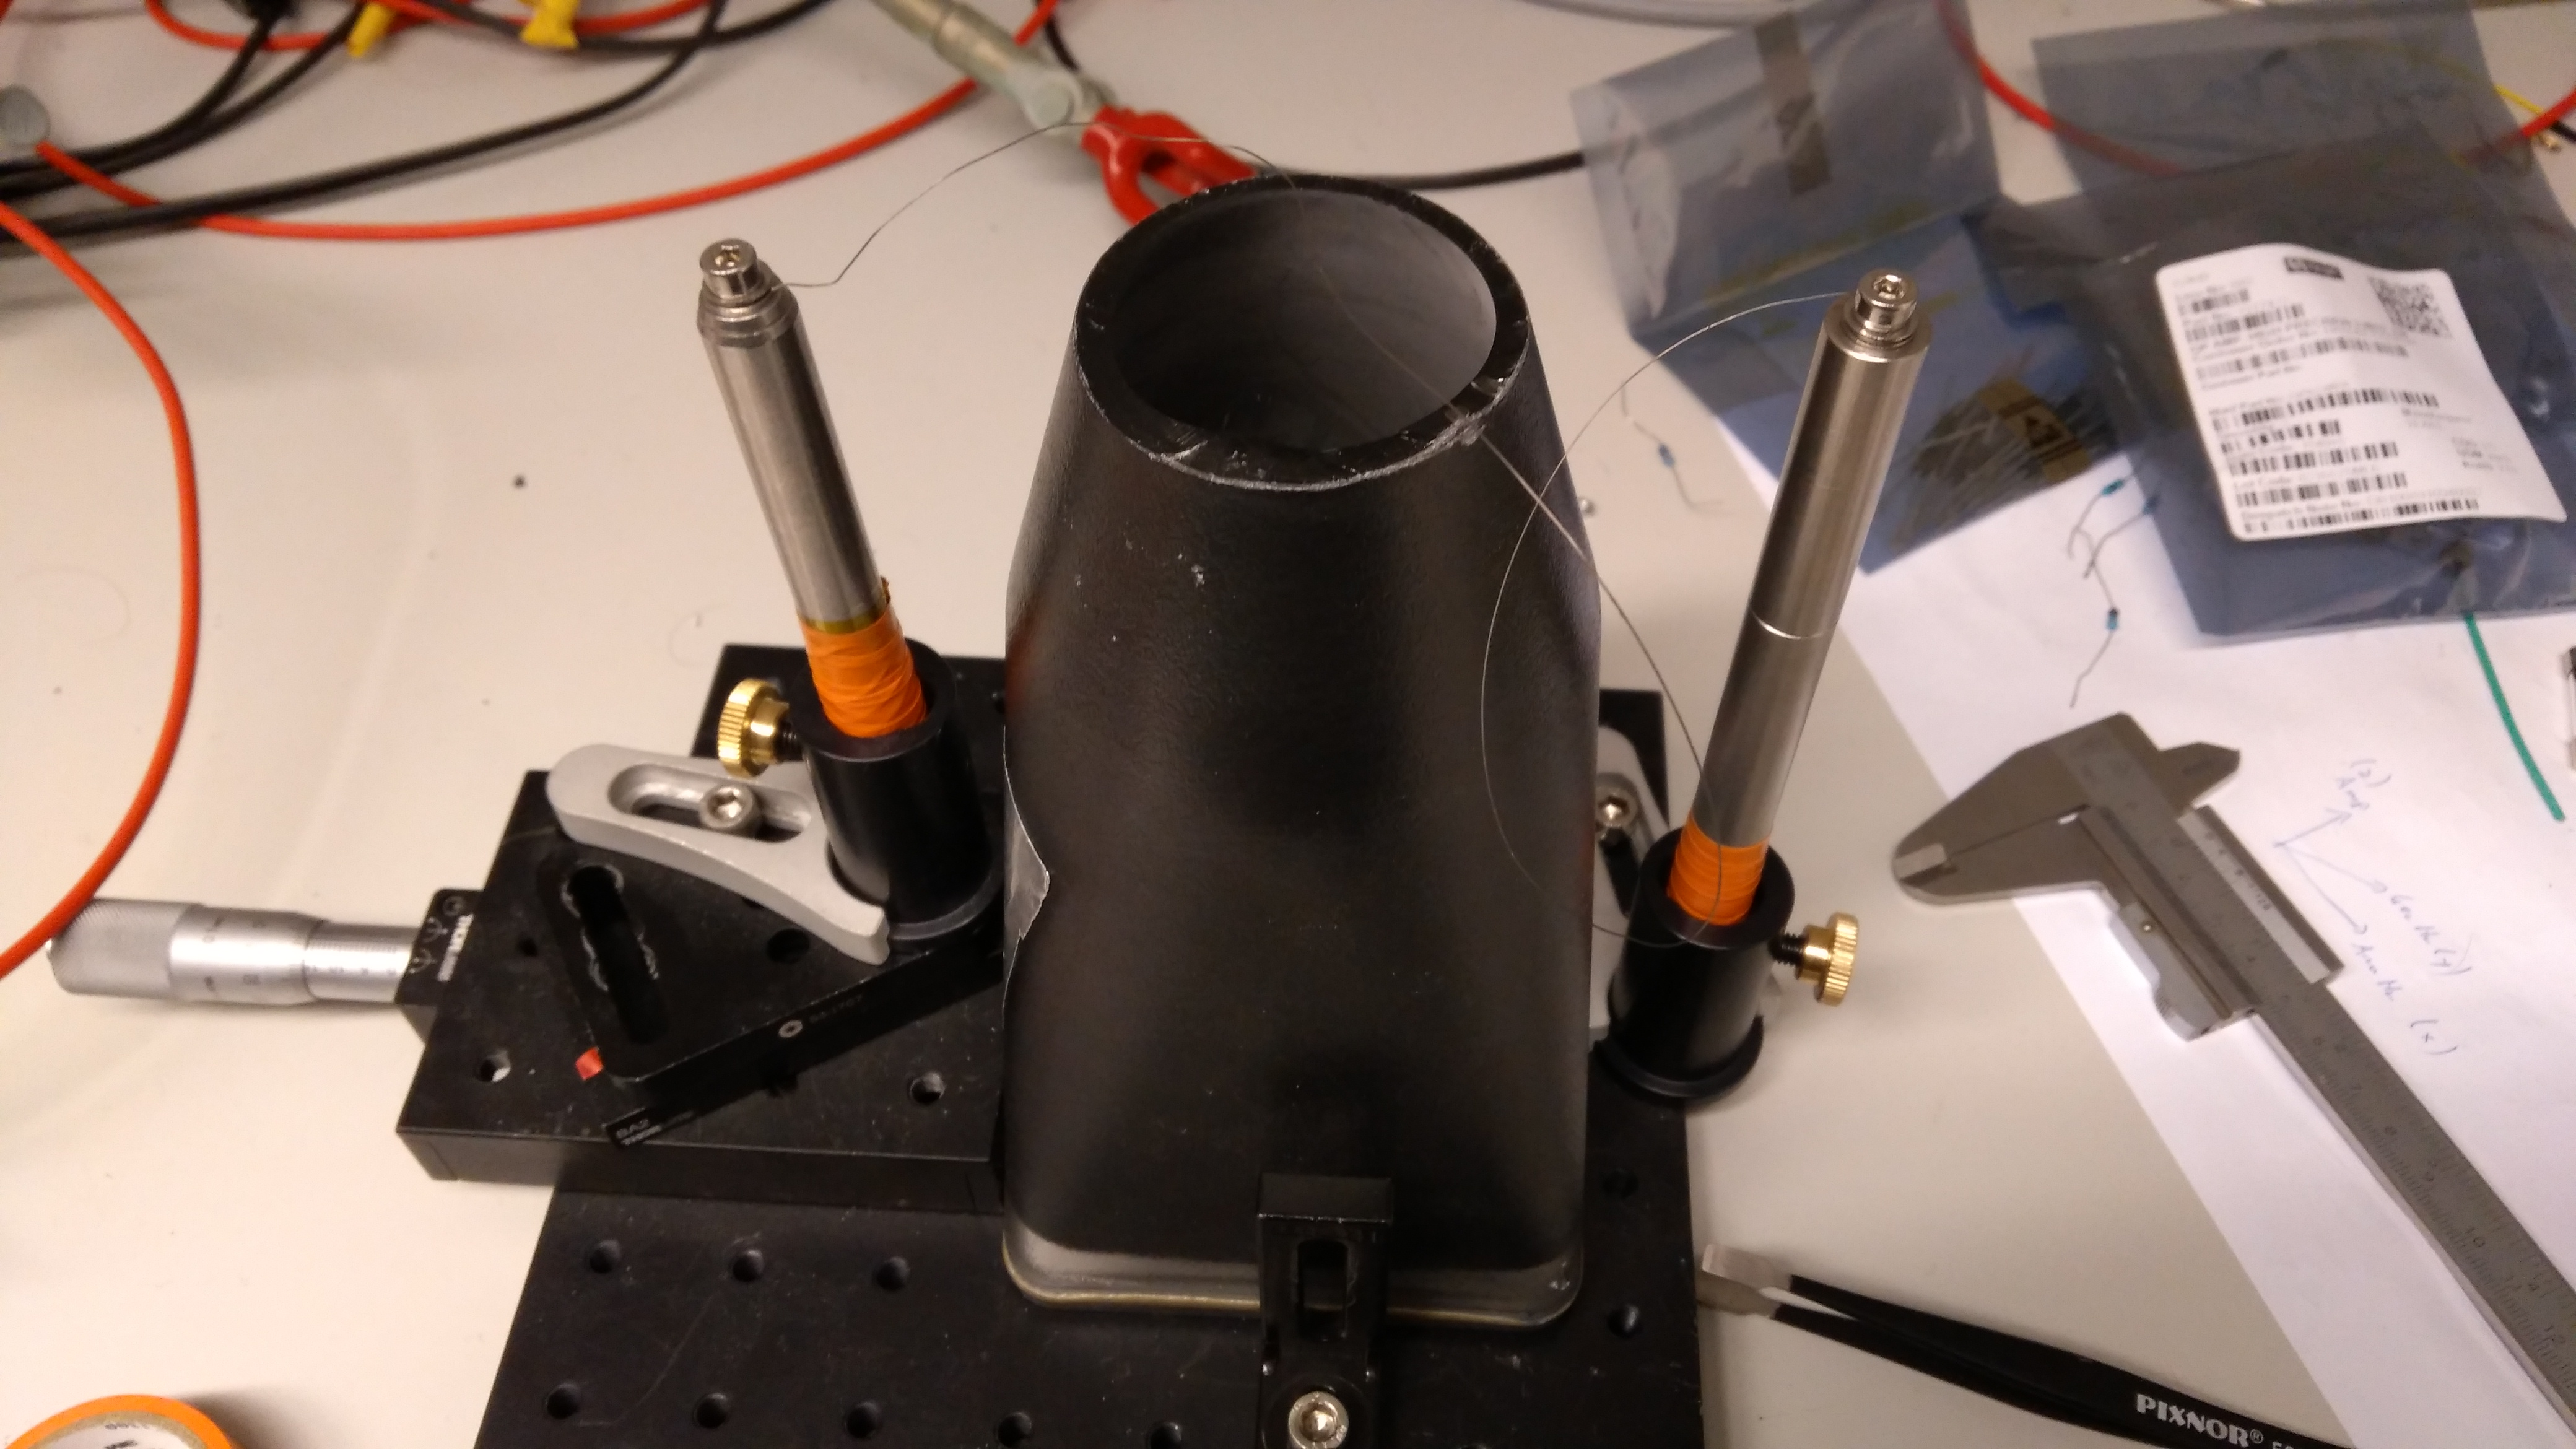
\includegraphics[width=.8\textwidth]{../Chapters/CRT-handling/Cutting_Stage.jpg}
	\end{figure}
\end{frame}

%------------------------------------------------
\section{Vacuum test chamber}

\begin{frame}
	\frametitle{3D rendering}
	\begin{figure}[ht]
		\centering
		
		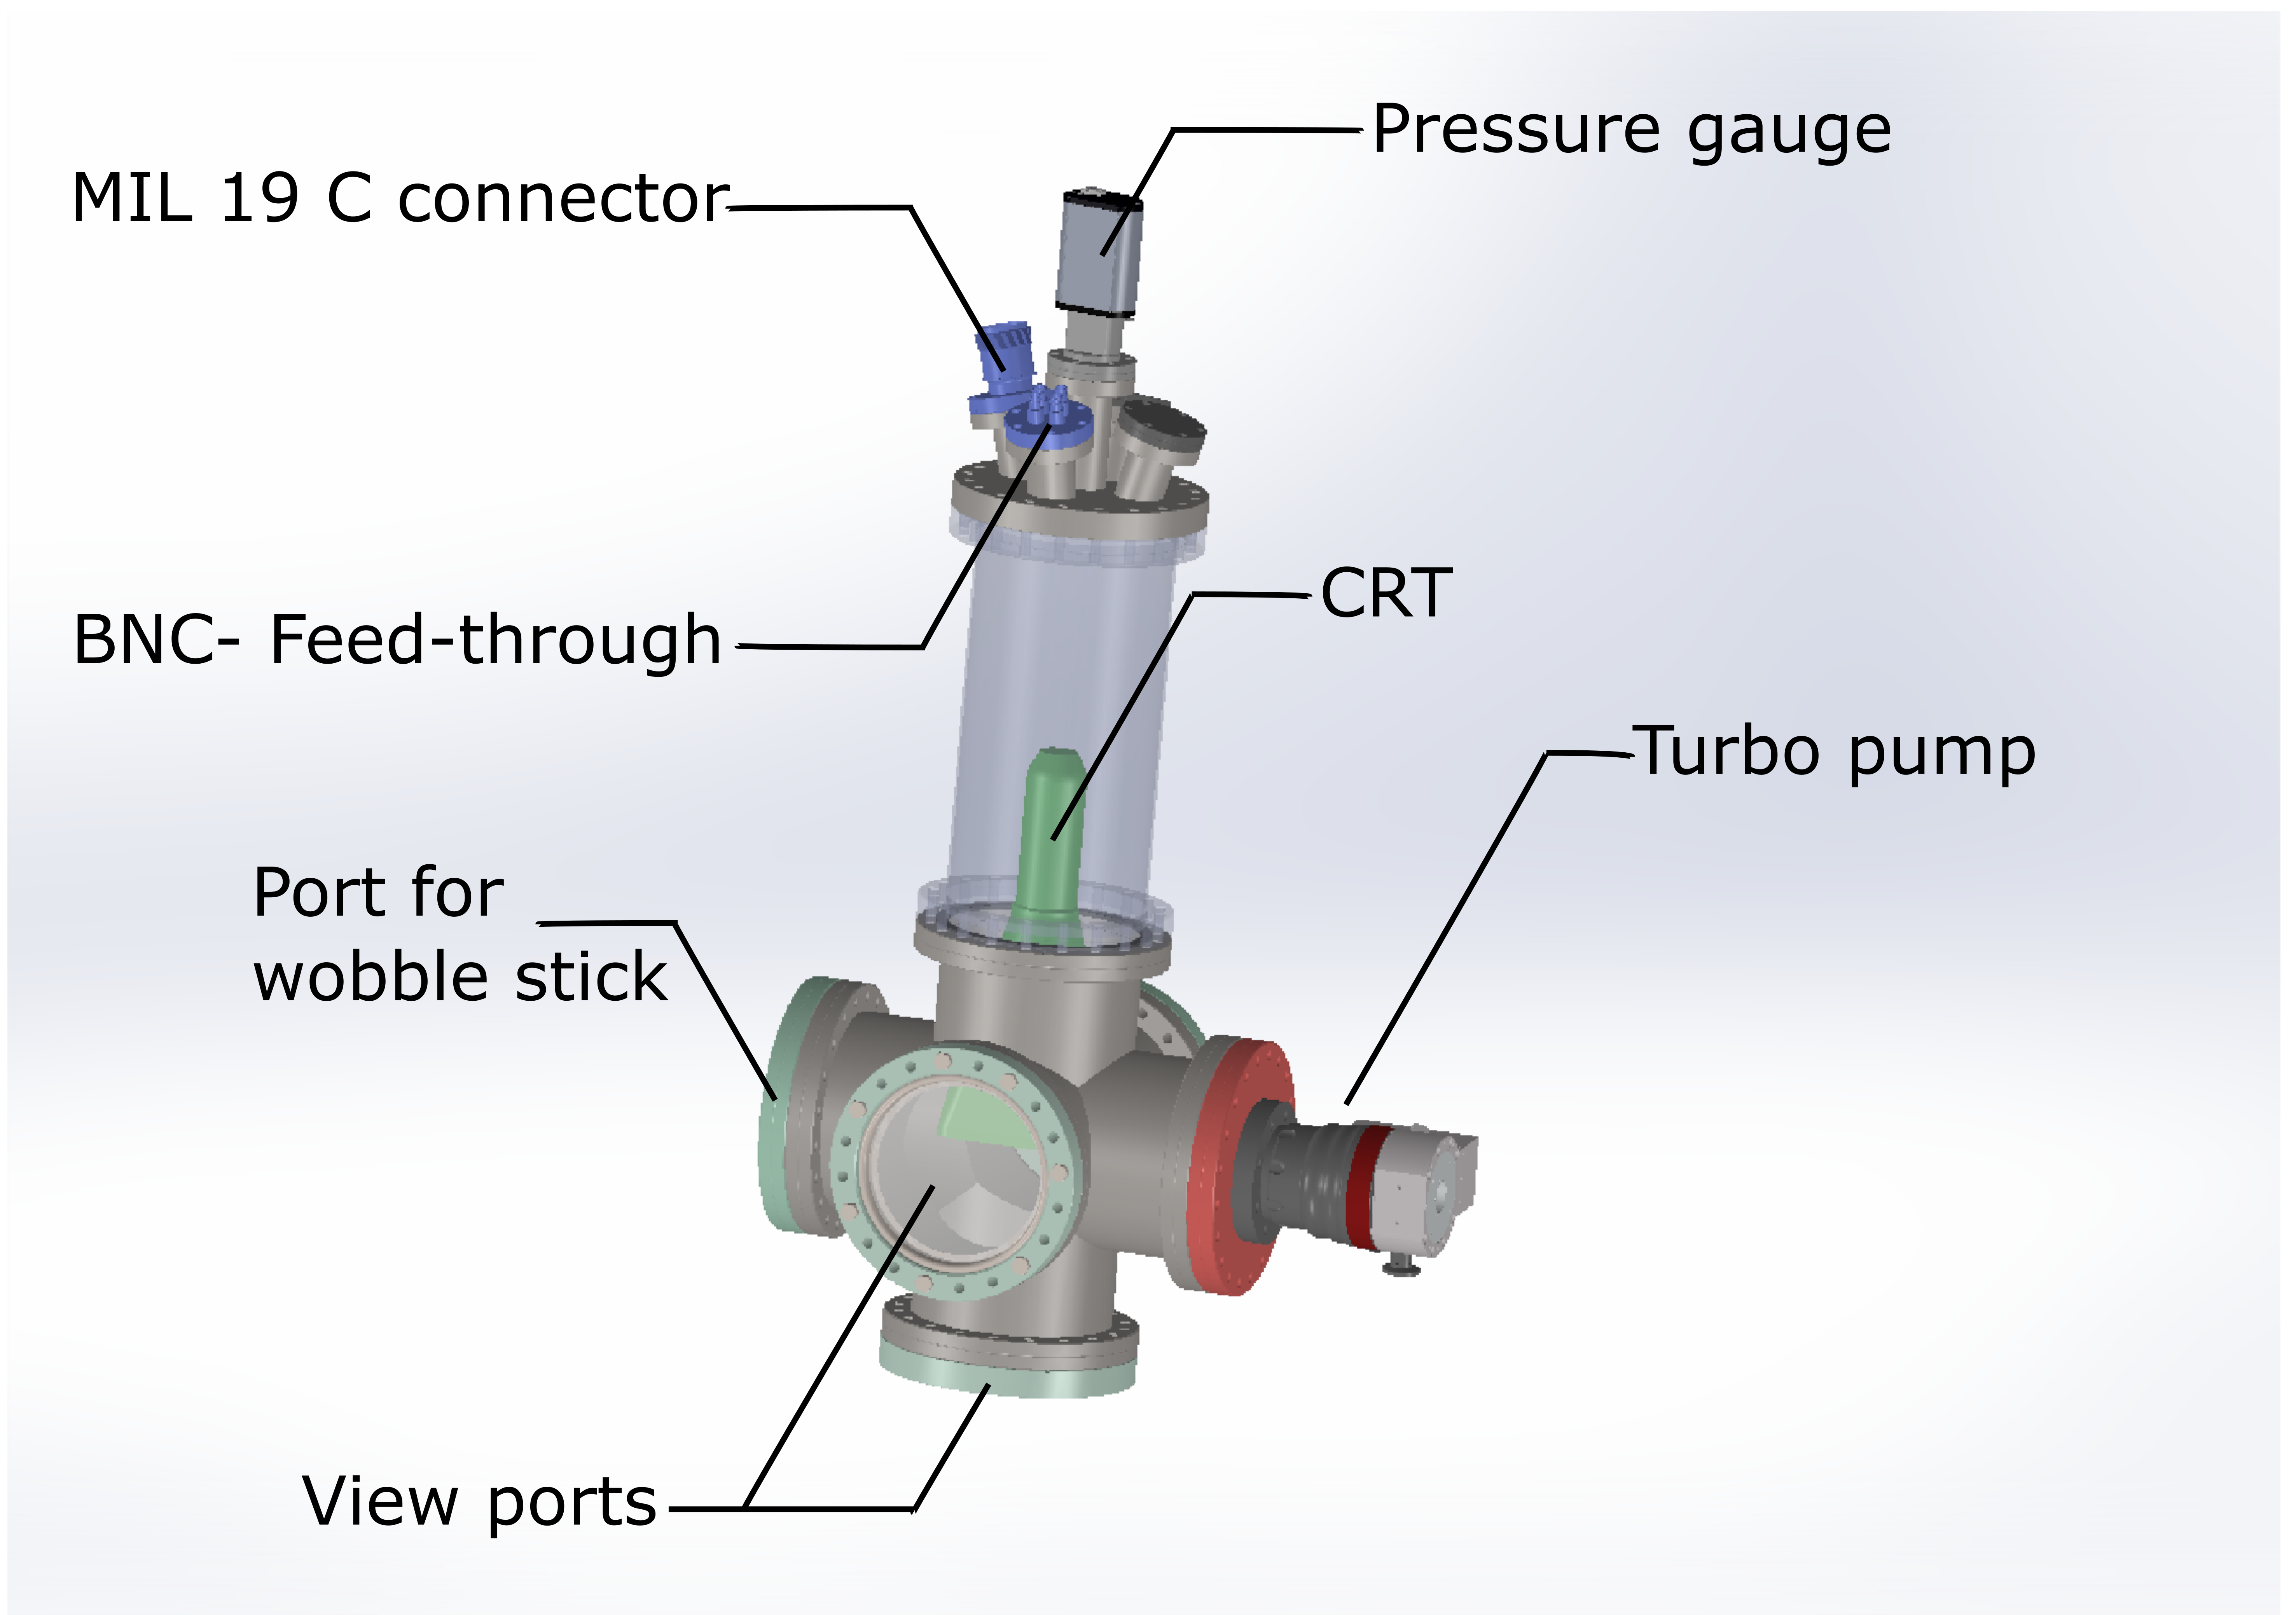
\includegraphics[width=0.65\textwidth]{../Chapters/vacuum-chamber/vacuum-chamber-annotated} % taken from OneNote QuaK/Vacuum Setup/Test vacuum chamber
	\end{figure}
\end{frame}

%------------------------------------------------
\section{Deflection Electronics}

\begin{frame}
	\frametitle{Deflection Electronics}
	\begin{figure}[ht]
		\centering
		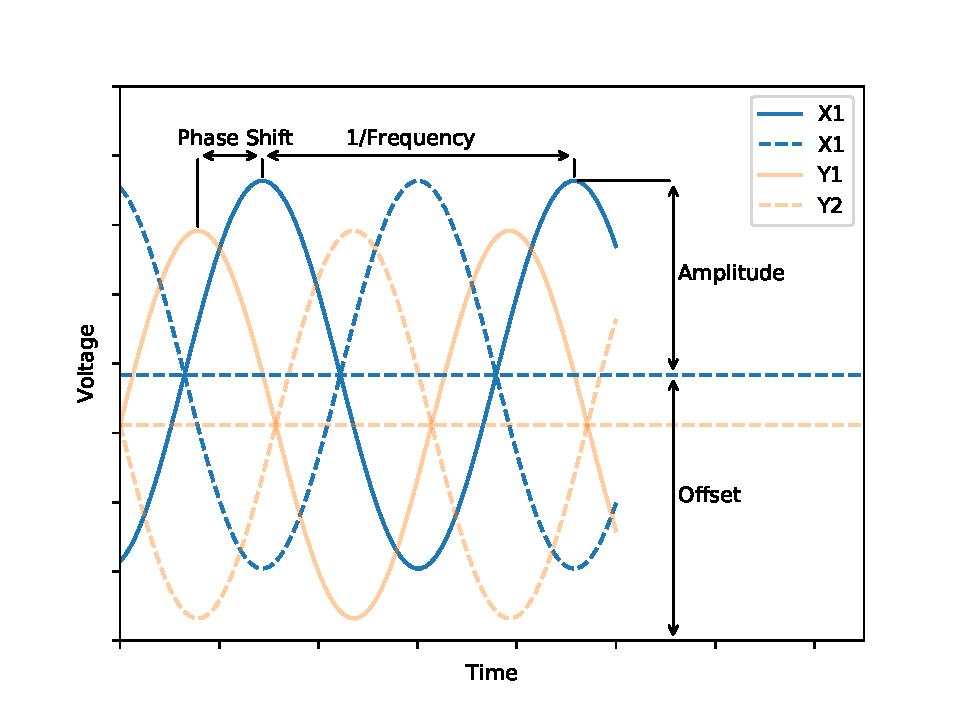
\includegraphics[width=0.8\textwidth]{../Chapters/Deflection/VoltageAspects}
	\end{figure}
\end{frame}

%------------------------------------------------

\begin{frame}
	\frametitle{Deflection circuit diagram}
	\begin{figure}[ht]
		\centering
		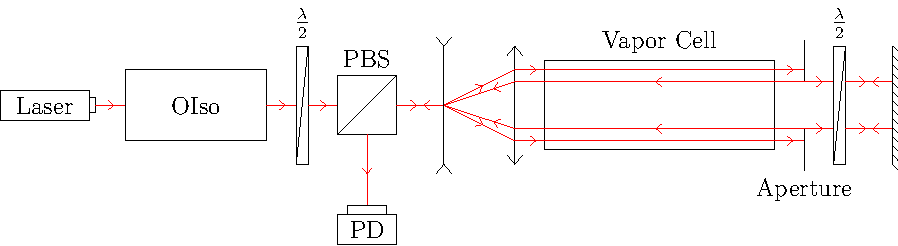
\includegraphics[width=0.9\textwidth]{../Figures/Thesis-figure2.pdf}
	\end{figure}
\end{frame}

%------------------------------------------------

\begin{frame}
	\frametitle{Measurements of center tapped transformer}
	\begin{figure}[ht]
		\centering
		\begin{subfigure}{0.4\textwidth}
			\centering
			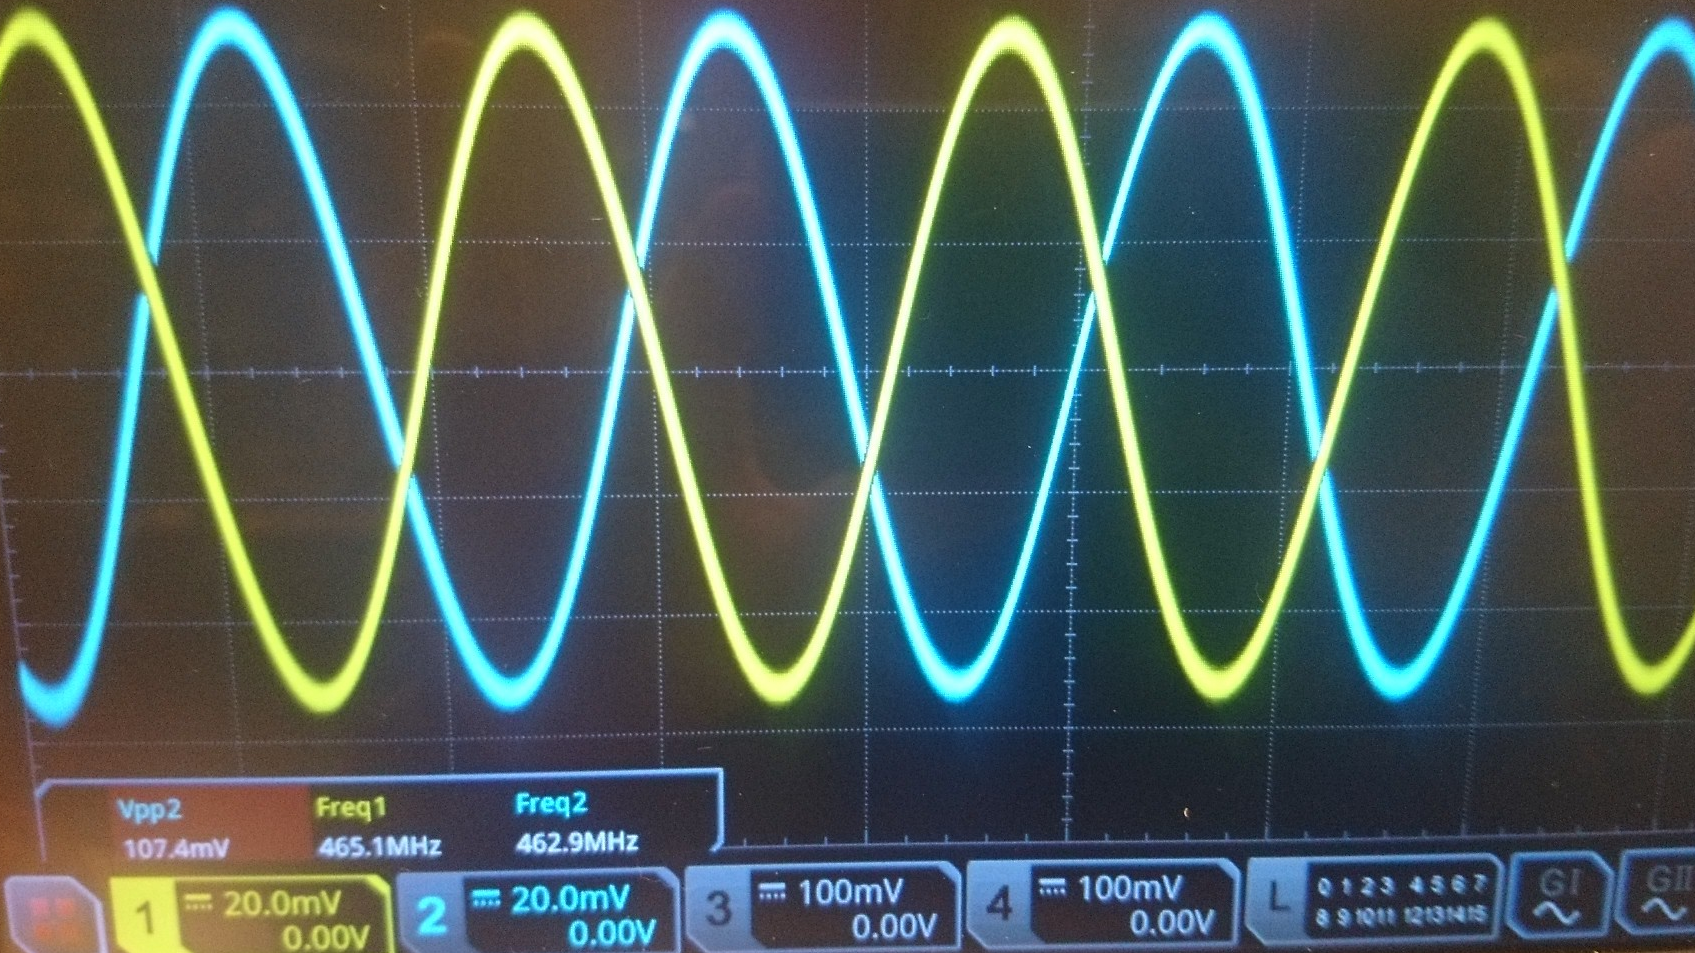
\includegraphics[width=\textwidth]{../Chapters/Deflection/unbiased3}
			\caption{Unbiased at \SI{465}{\mega\hertz}}
		\end{subfigure}
		\hspace{0.1\textwidth}
		\begin{subfigure}{0.4\textwidth}
			\centering
			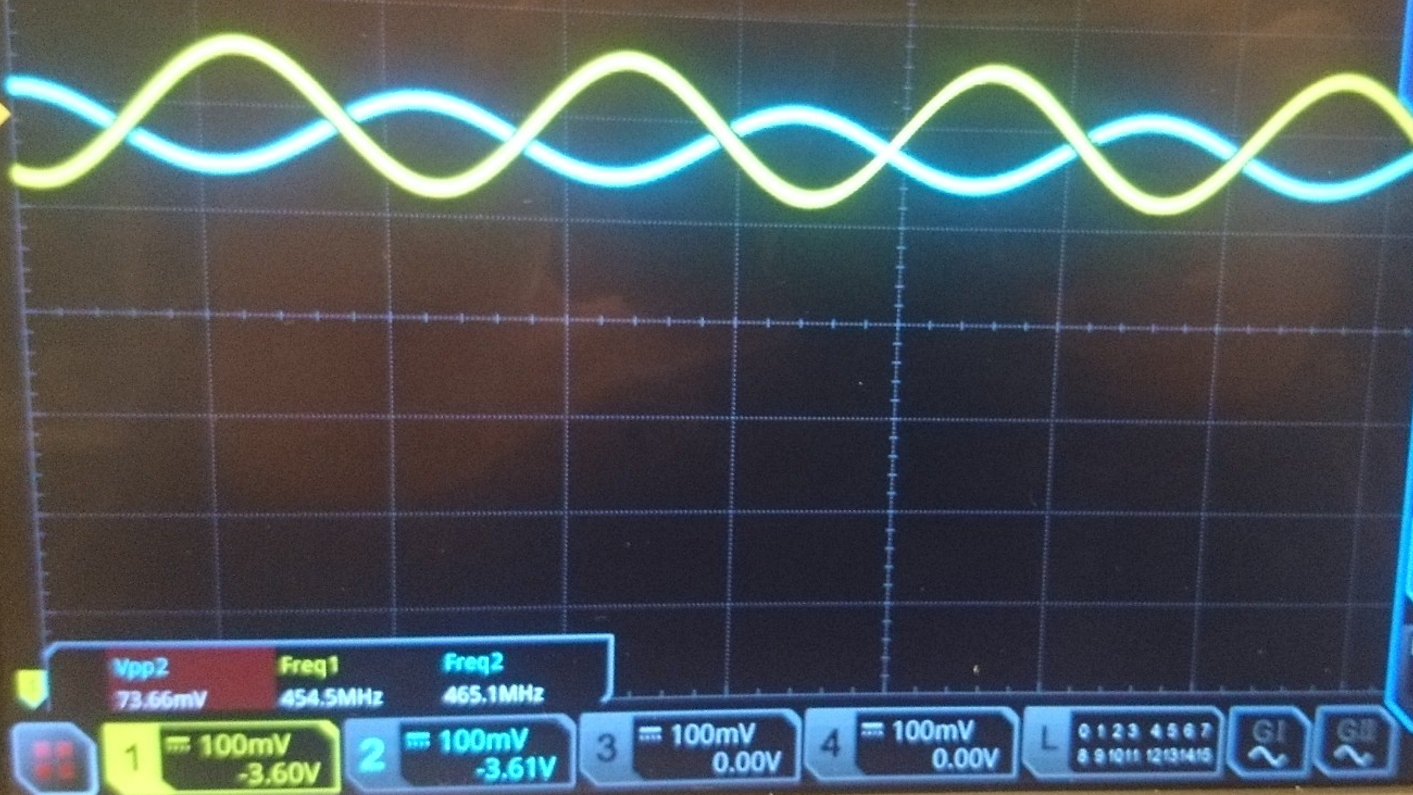
\includegraphics[width=\textwidth]{../Chapters/Deflection/biased3}
			\caption{Biased at \SI{465}{\mega\hertz}}
		\end{subfigure}
	\end{figure}
\end{frame}

%------------------------------------------------
\section{Beam characterization}

\begin{frame}
	\frametitle{First measurements of e-beam}
	\begin{figure}[h]
		\centering
		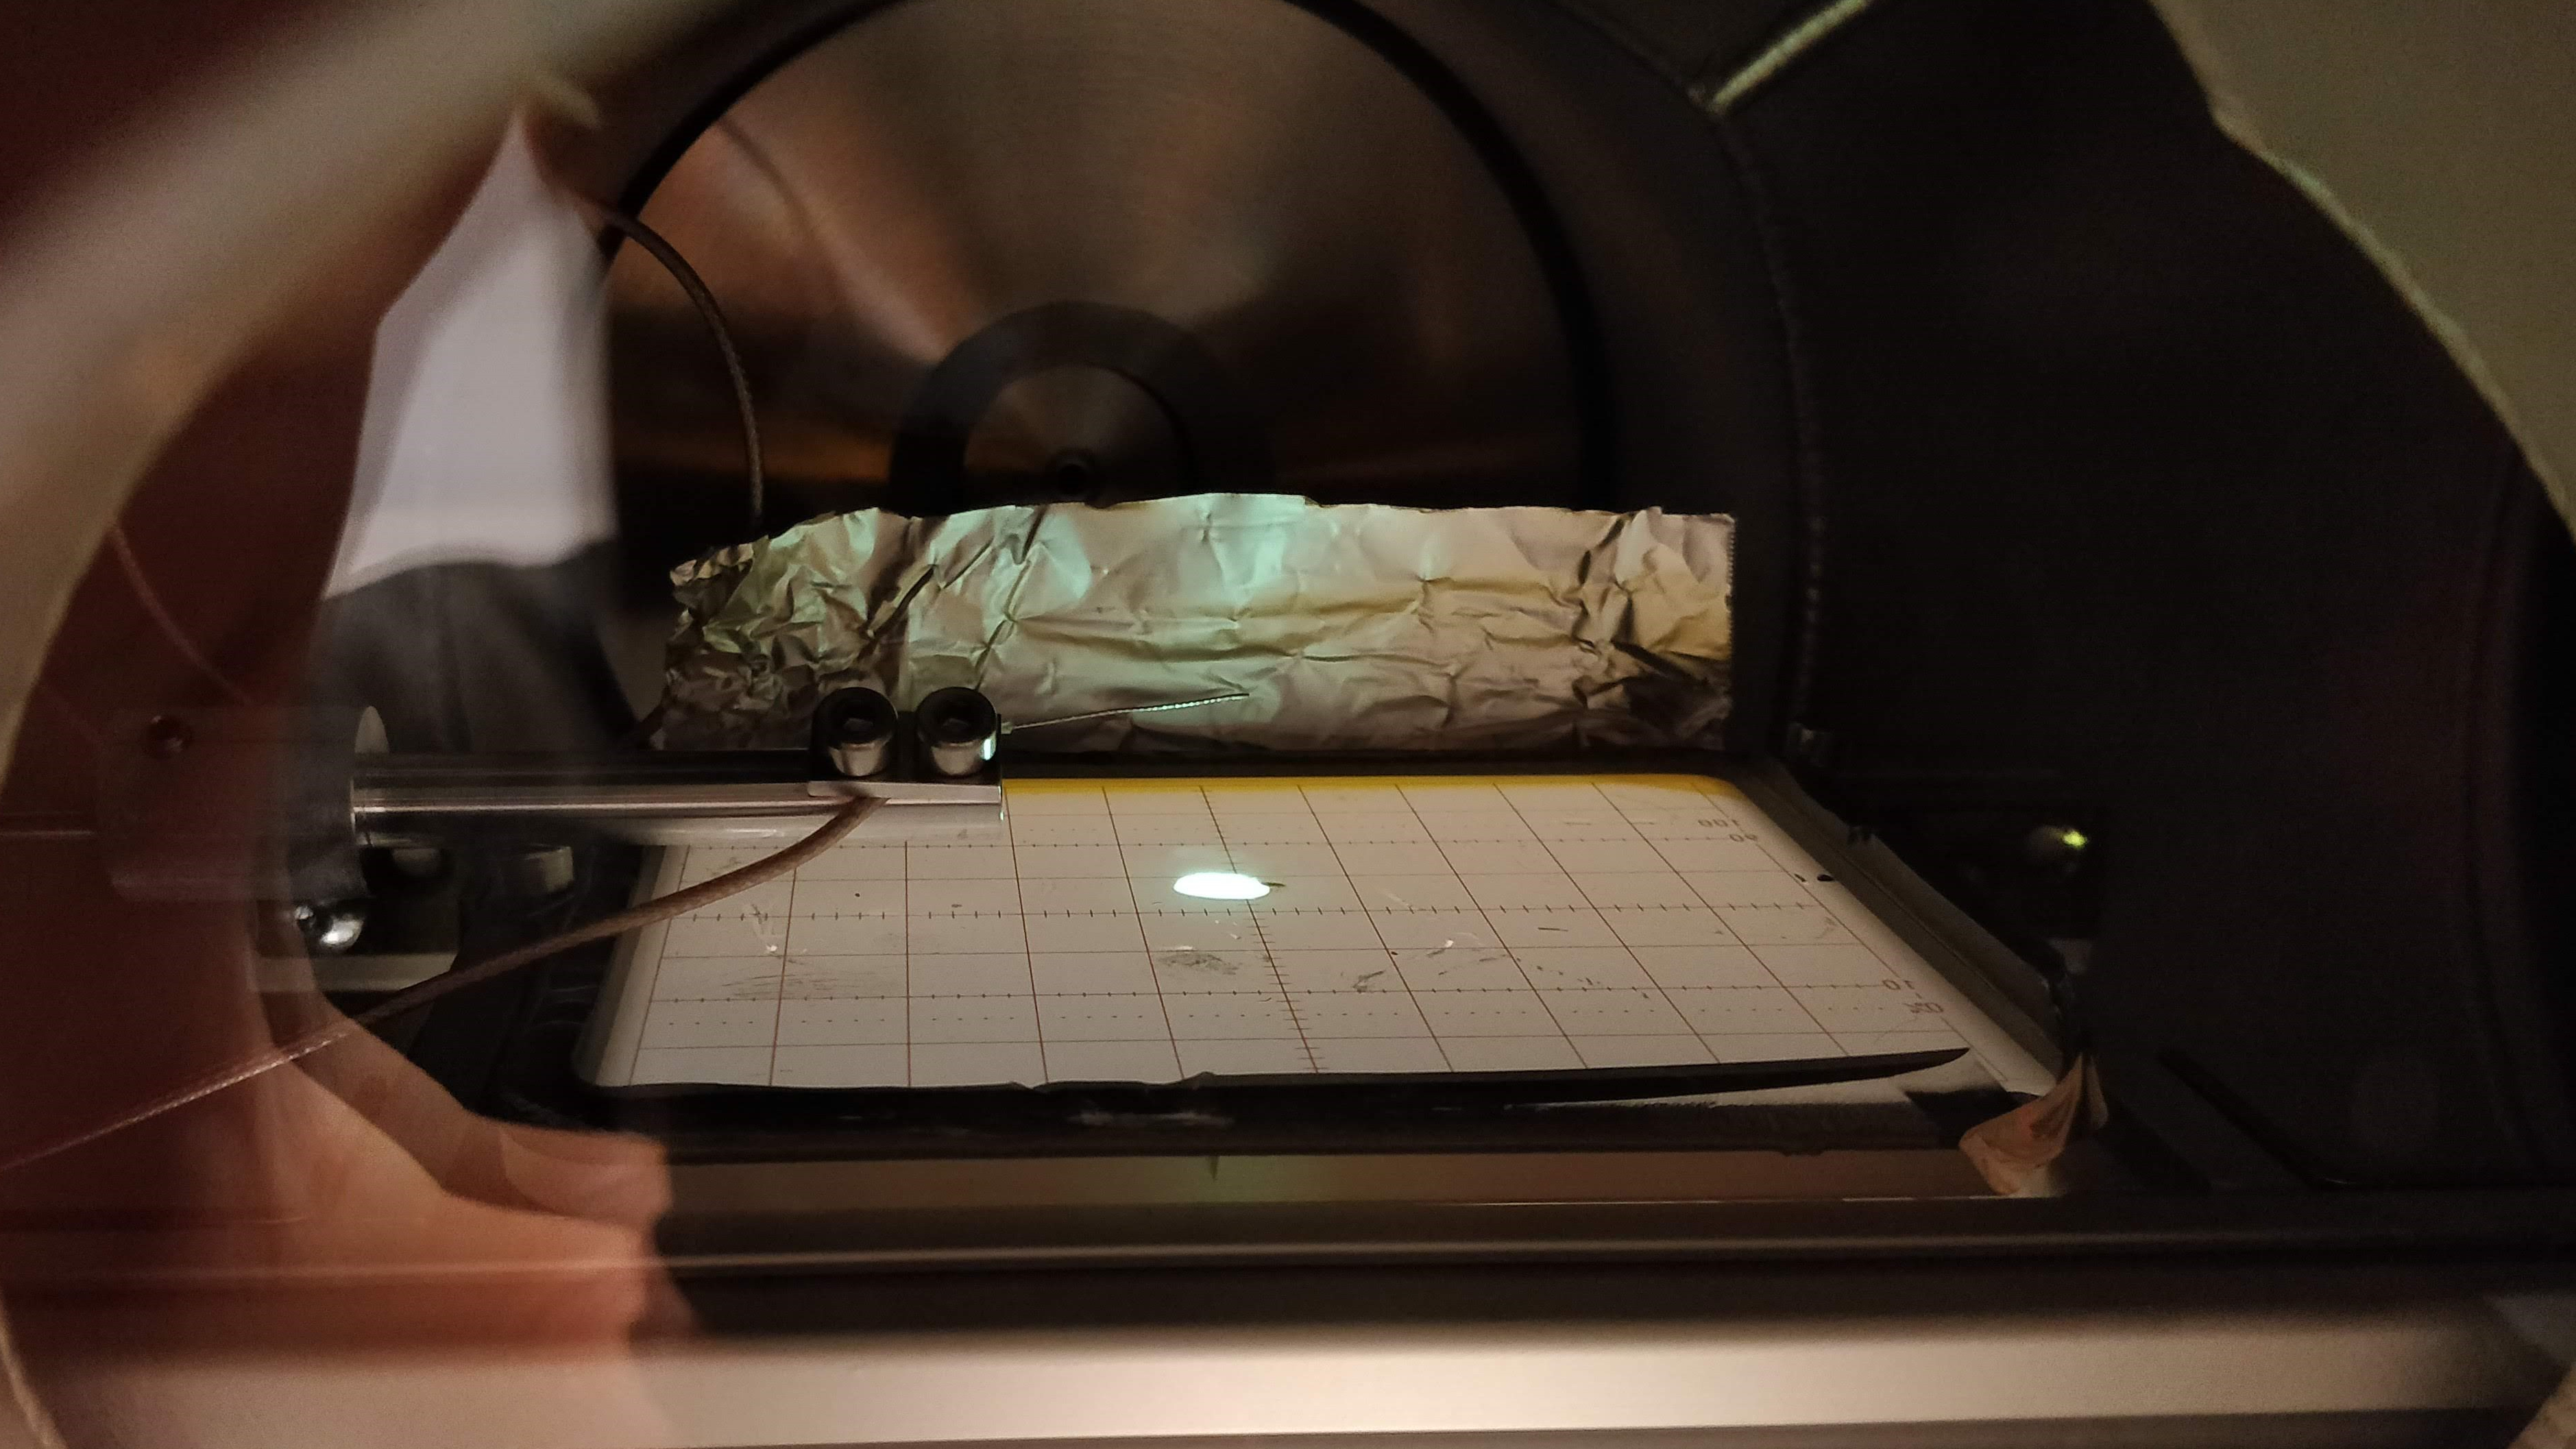
\includegraphics[width=0.8\textwidth]{../Chapters/beam-characterization/center_image}
	\end{figure}
\end{frame}

%------------------------------------------------

\begin{frame}
	\frametitle{Measured beam current (aluminum)}
	\begin{figure}[h]
		\centering
		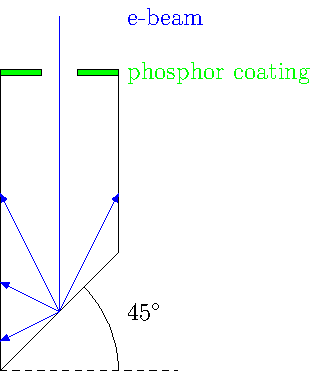
\includegraphics[width=0.9\textwidth]{../Figures/Thesis-figure3.pdf}
	\end{figure}
\end{frame}

%------------------------------------------------

\begin{frame}
	\frametitle{Schematics Faraday cup}
	\begin{figure}[h]
		\centering
		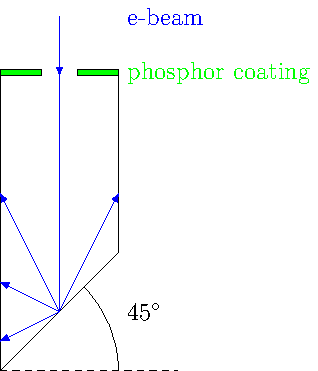
\includegraphics[width=0.4\textwidth]{../Figures/Thesis-figure4.pdf}
	\end{figure}
\end{frame}

%------------------------------------------------

\begin{frame}
	\frametitle{Measured beam current (cup)}
	\begin{figure}[h]
		\centering
		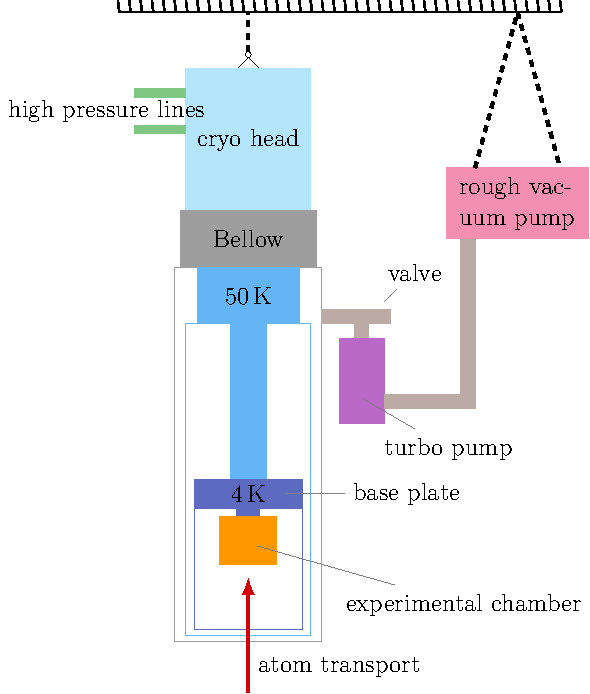
\includegraphics[width=0.6\textwidth]{../Figures/Thesis-figure5.pdf}
	\end{figure}
\end{frame}
%------------------------------------------------

\begin{frame}
	\frametitle{Measurement of deflection frequency}
	\begin{figure}
		\centering
		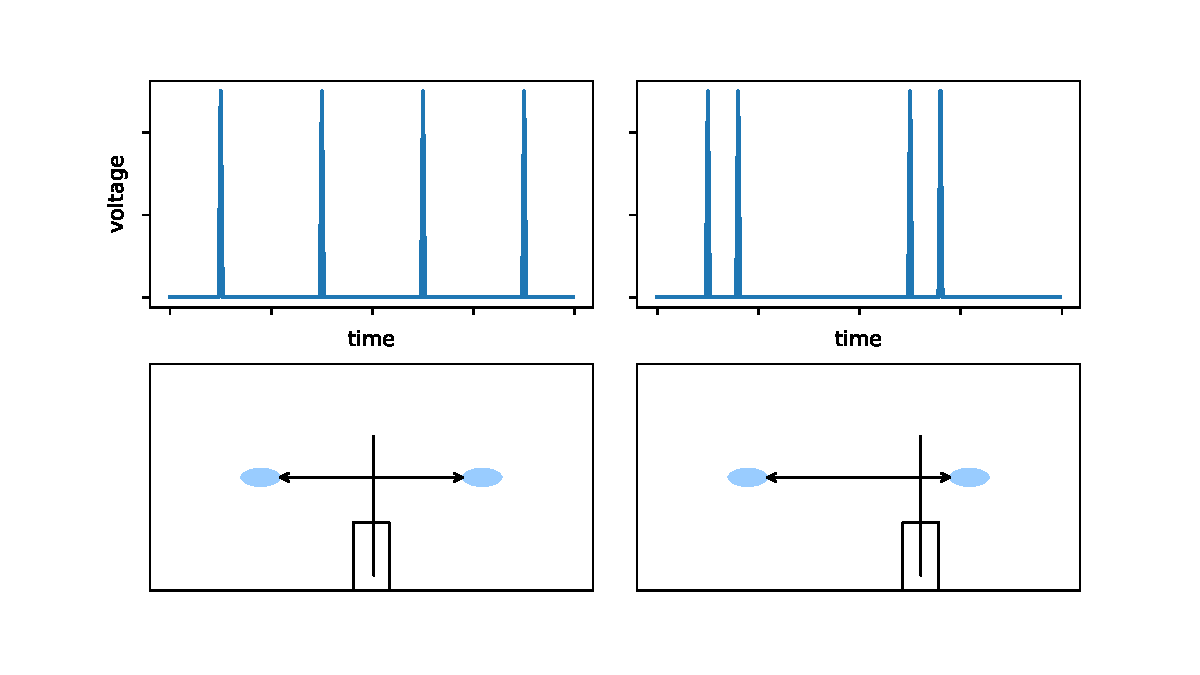
\includegraphics[width=0.8\linewidth]{../Chapters/beam-characterization/Spikes}
	\end{figure}
\end{frame}

%------------------------------------------------

\begin{frame}
\Huge{\centerline{Thank you for your attention!}}
\end{frame}

%----------------------------------------------------------------------------------------

\end{document} 